\documentclass{article}

\usepackage[top=0.6in, bottom=0.75in, left=0.625in, right=0.625in]{geometry}
\usepackage{amsmath,amsthm,amssymb,hyperref}
\usepackage[utf8x]{inputenc}
\usepackage[russianb]{babel}
\usepackage{hyperref}
% \usepackage{minted}
\usepackage{color}
\usepackage{fancyhdr}


\newcommand{\R}{\mathbb{R}}  
\newcommand{\Z}{\mathbb{Z}}
\newcommand{\N}{\mathbb{N}}
\newcommand{\Q}{\mathbb{Q}}
\newcommand{\tu}[1]{\underline{#1}}
\newcommand{\tb}[1]{\textbf{#1}}
\newcommand{\ti}[1]{\textit{#1}}
\newcommand{\aliq}{\mathrel{\raisebox{-0.5ex}{\vdots}}}
\newcommand{\mylim}[2]{\lim_{#1 \to #2}}
\newcommand{\abs}[1]{\left|{#1}\right|}
\newcommand{\brackets}[1]{\left({#1}\right)}
\newcommand{\sqbrackets}[1]{\left[{#1}\right]}

\newenvironment{theorem}[2][Theorem]{\begin{trivlist}
\item[\hskip \labelsep {\bfseries #1}\hskip \labelsep {\bfseries #2.}]}{\end{trivlist}}
\newenvironment{lemma}[2][Lemma]{\begin{trivlist}
\item[\hskip \labelsep {\bfseries #1}\hskip \labelsep {\bfseries #2.}]}{\end{trivlist}}
\newenvironment{claim}[2][Claim]{\begin{trivlist}
\item[\hskip \labelsep {\bfseries #1}\hskip \labelsep {\bfseries #2.}]}{\end{trivlist}}
\newenvironment{problem}[2][Problem]{\begin{trivlist}
\item[\hskip \labelsep {\bfseries #1}\hskip \labelsep {\bfseries #2.}]}{\end{trivlist}}
\newenvironment{proposition}[2][Proposition]{\begin{trivlist}
\item[\hskip \labelsep {\bfseries #1}\hskip \labelsep {\bfseries #2.}]}{\end{trivlist}}
\newenvironment{corollary}[2][Corollary]{\begin{trivlist}
\item[\hskip \labelsep {\bfseries #1}\hskip \labelsep {\bfseries #2.}]}{\end{trivlist}}

\newenvironment{solution}{\begin{proof}[Solution]}{\end{proof}}

\makeatletter
\newenvironment{sqcases}{%
  \matrix@check\sqcases\env@sqcases
}{%
  \endarray\right.%
}
\def\env@sqcases{%
  \let\@ifnextchar\new@ifnextchar
  \left\lbrack
  \def\arraystretch{1.2}%
  \array{@{}l@{\quad}l@{}}%
}
\makeatother

\ifx\pdfoutput\undefined
\usepackage{graphicx}
\else
\usepackage[pdftex]{graphicx}
\fi

\pagestyle{fancy}
\fancyhf{}
\fancyhead[LE,RO]{Макоян Артем, ПМИ 191-1, @MakArtKar, \href{http://github.com/MakArtKar}{\textcolor{blue}{github}}, \href{http://codeforces.com/profile/MakArtKar}{\textcolor{blue}{codeforces}}, \href{vk.com/makartkar}{\textcolor{blue}{vk}}}
\fancyhead[RE,LO]{Лекция по АиСД 28.11}

\begin{document}

\tu{Куча}: insert, extract\_min, decrease\_min, decrease\_key, increase\_key, merge. Хотим добавить операцию merge - объединить 2 кучи. Считаем, что можем делать операции амортизировано (не разделяем кучи и кучи не персистентные). Меньшую кучу будем добавлять в большую ("переливать" в большую). 

Хотелось бы раздать каждой вершине по $\log n$ монет и говорить, что, когда мы "переливаем" кучу, все элементы этой кучи платят по монете. Тогда монет хватит, так как при каждом переливании размер кучи, где находится вершина увеличивается вдвое, значит каждая вершина перельется не более $\log n$ раз. Но все ломается из-за того, что мы можем удалять вершины. Можно ввести потенциалы (подумать), а можно сказать, что у каждого элемента есть ранг (r(i)) и при каждом переливании все ранги меньшей кучи увеличиваются на 1. Тогда амортизировано merge будет работать за O($\log^2 n$). \\

\tu{Биномиальная куча}: \\

Вершин в биномиальной кучи $2^n$, на $k$-ом слое $C_n^k$ вершин. Из каждой вершины храним ребро в старшего сына, в предка и в следующего брата. $B_k = $ merge$(B_{k-1}, B_{k-1})$. %вставить картинку 
Заметим, что merge деревьев одного ранга работает за O(1). \\

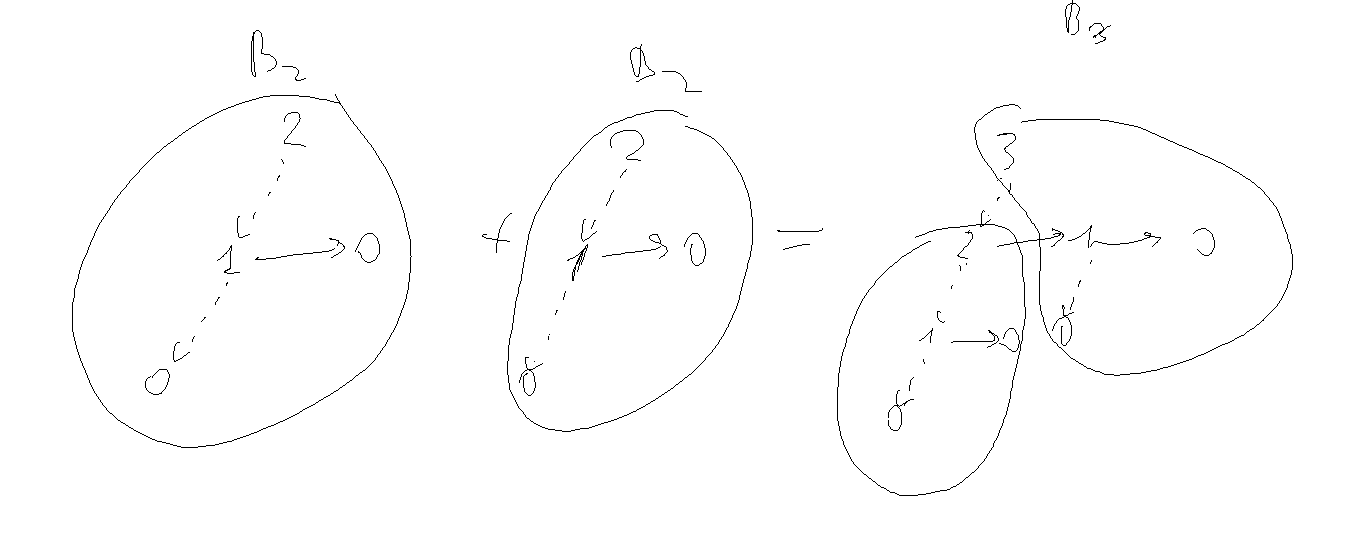
\includegraphics[width=15cm]{../pictures/binominial_heap_add.png}


Если у нас есть n чисел, то как мы их поместим в кучу размера $2^k$? $n = 2^{k_1} + 2^{k_2} \dots + 2^{k_m}$. Тогда можем хранить все элементы как кучи рангов $k_1, \dots k_m$. Тогда при merge нужно объединять два списка биномиальных куч (будем делать это 2 указателями по 2 массивам), будем объединять кучи одинаковых рангов \\ %вставить картинку или объяснение

insert - создаем кучу ранга 0 с нашим элементом и делаем merge за $O(\log n$).

Для поиска минимума будем просто поддерживать глобальный минимум, изменяя его за O($\log n$) (пробегаясь по всем кучам) при каждом запросе изменения. \\

decrease\_key \\

extract\_min \\

increase\_key: decrease\_key(v, $-\infty$) $\to$ extract\_min $\to$ insert(x). Работает за O($\log n$). \\ 

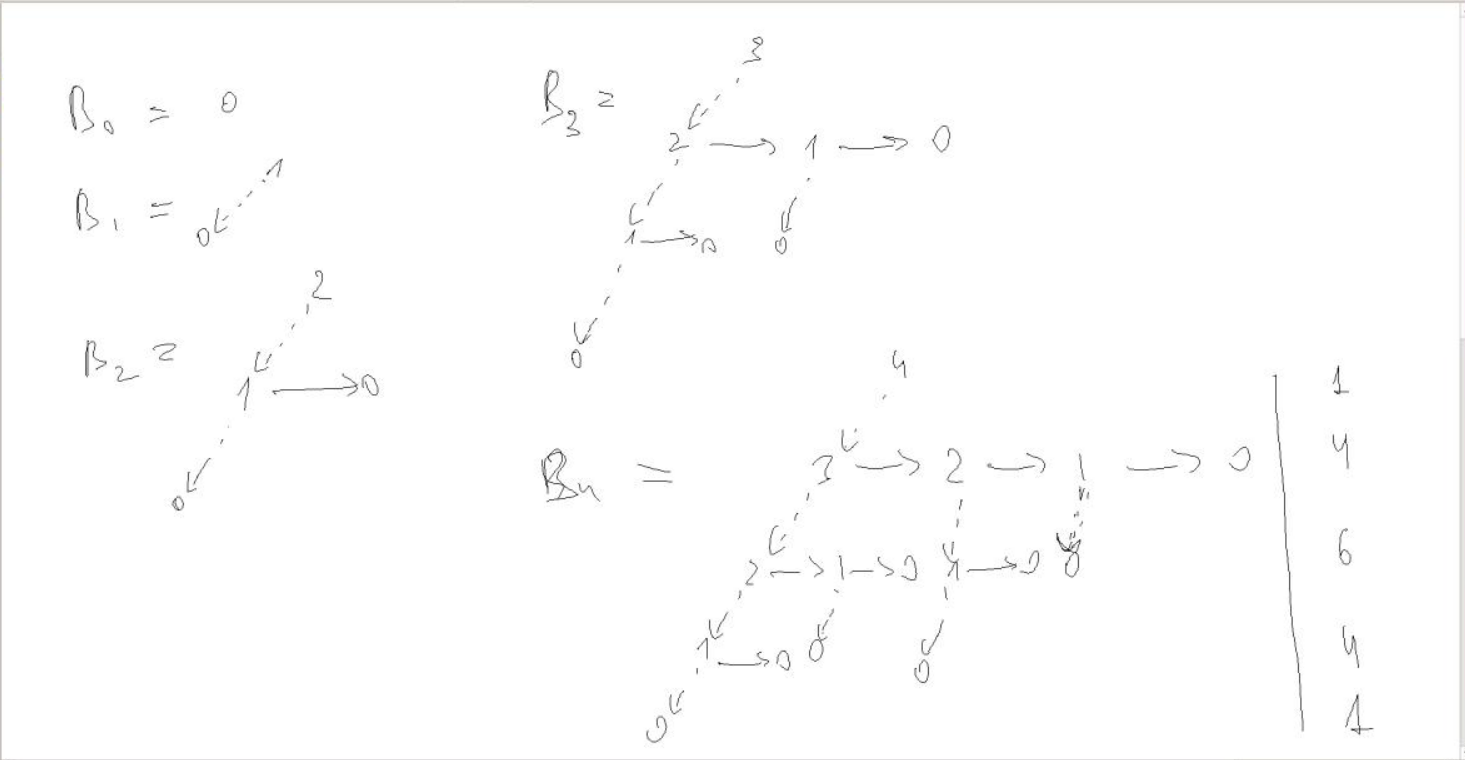
\includegraphics[width=15cm]{../pictures/binominial_heap.png}

\tu{Фибоначчиева куча}: (чет я устал техать, чекайте у Кости)

\begin{center}
\begin{tabular}{|c|c|c|c|}
\hline
Операции        &   binary heap             & binomial heap & fibonacci heap        \\
\hline
insert          &   O($\log n$)             & O($\log n$)   & O(1)                  \\
extract\_min    &   O($\log n$)             & O($\log n$)   & $\tilde{O}(\log n)$   \\
decrease\_min   &   O($\log n$)             & O($\log n$)   & $\tilde{O}(1)$        \\
increase\_min   &   O($\log n$)             & O($\log n$)   & $\tilde{O}(\log n)$   \\
merge           &   $\tilde{O}(\log^2 n)$   & O($\log n$)   & O(1)                  \\
get\_min        &   O(1)                    & O(1)          & O(1)                  \\
\hline
\end{tabular}
\end{center}



\end{document}